\jxhj{%教学后记
	}
\skrq{%授课日期
2017年3月27日 4-5节	}
\ktmq{%课题名称
	 局部坐标系}
\jxmb{%教学目标,每行前面要加 \item
	\item 掌握Fanuc上G52指令的格式;
	\item 掌握Siemens上Trans指令的格式;
	\item 掌握用局部坐标系指令编程。 }
\jxzd{%教学重点,每行前面要加 \item
	\item Fanuc上G52指令的格式;
	\item 用局部坐标系指令编程。 }
\jxnd{%教学难点,每行前面要加 \item
	\item 用局部坐标系指令编程。 }
\jjff{%教学方法
	通过讲述、举例、演示法来说明;}

\makeshouye %制作教案首页

%%%%教学内容
\subsection{组织教学}
\begin{enumerate}[\hspace{2em}1、]
	\item 集中学生注意力;
	\item 清查学生人数;
	\item 维持课堂纪律;
\end{enumerate}
\subsection{复习导入及主要内容}
\begin{enumerate}[\hspace{2em}1、]
\item 相关内容;
\item 椭圆弧加工;
\item 应用实例;
\end{enumerate}


\subsection{教学内容及过程}
\subsubsection{几种坐标系}
\paragraph{工件坐标系}
G54-G59、G92

G54-G59是在机床参数中以机床坐标为基准设定工件坐标系

G92是在程序中以刀具当前位置为基准设定工件坐标系

一般使用G54~G59指令后,就不再使用G92指令。

\paragraph{机床坐标系}
G53

当需要用机床坐标系编程时,用G53指令。

机床坐标系通过回零(回参考点)建立。

如坐标系不对,可通过回零重新建立机床坐标系,机床坐标系原点在机床上是固定的一个点,这个点不会变的。
\paragraph{局部坐标系}
G52、Trans

在工件坐标上建立一个子工件坐标系。即局部坐标系。
\subsubsection{Fanuc上局部坐标系}
指令格式:  G52 X\_ Y\_ Z\_;建立局部坐标系

G52 X0 Y0 Z0 ;取消局部坐标系。

说明:其X、Y的定义是原坐标系的程序原点到子坐标系的程序原点之向量值。

G52 X0 Y0;=>表示回复到原坐标系。

注意:
\begin{enumerate}[\hspace{2em}A、]
	\item 局部坐标系设定不改变工件和机床坐标系。 
\item 当用G50定义工件坐标系时,如果没有对局部坐标系中的所有轴指定坐标值,局部坐标系保持不变。
如果没有为局部坐标系中的任何轴指定坐标值,局部坐标系被取消。 
\item G52暂时取消刀尖半径补偿中的偏移。 
\item 在绝对方式紧跟G52之后指令一个运动指令。 
\item 复位时是否取消局部坐标系取决于参数的设定。当3402号参数的第6位(CLR)或者1202号参数3位(RLC)设为1时,局部坐标系在复位状态被取消。 
\item 手动返回参考点是否取消局部坐标系取决于ZCL的设定(参数1201的第2位)。
\end{enumerate}
\subsubsection{Siemens上的局部坐标系}
指令格式:

TRANS X\_ Y\_ Z\_ ;可编程的偏移,清除所有有关偏移、旋转、比例系数、镜像的指令 

ATRANS X\_ Y\_ Z\_ ;可编程的偏移,附加于当前的指令 

TRANS;不带数值清除所有有关偏移、旋转、比例系数、镜像的指令 

TRANS/ATRANS 指令要求一个独立的程序段。

\subsubsection{编程实例}
在数控机床上加工如图\ref{局部坐标系}所示的零件,完成工艺分析及加工程序的编写。

\begin{figure}[!hbtp]
	\centering	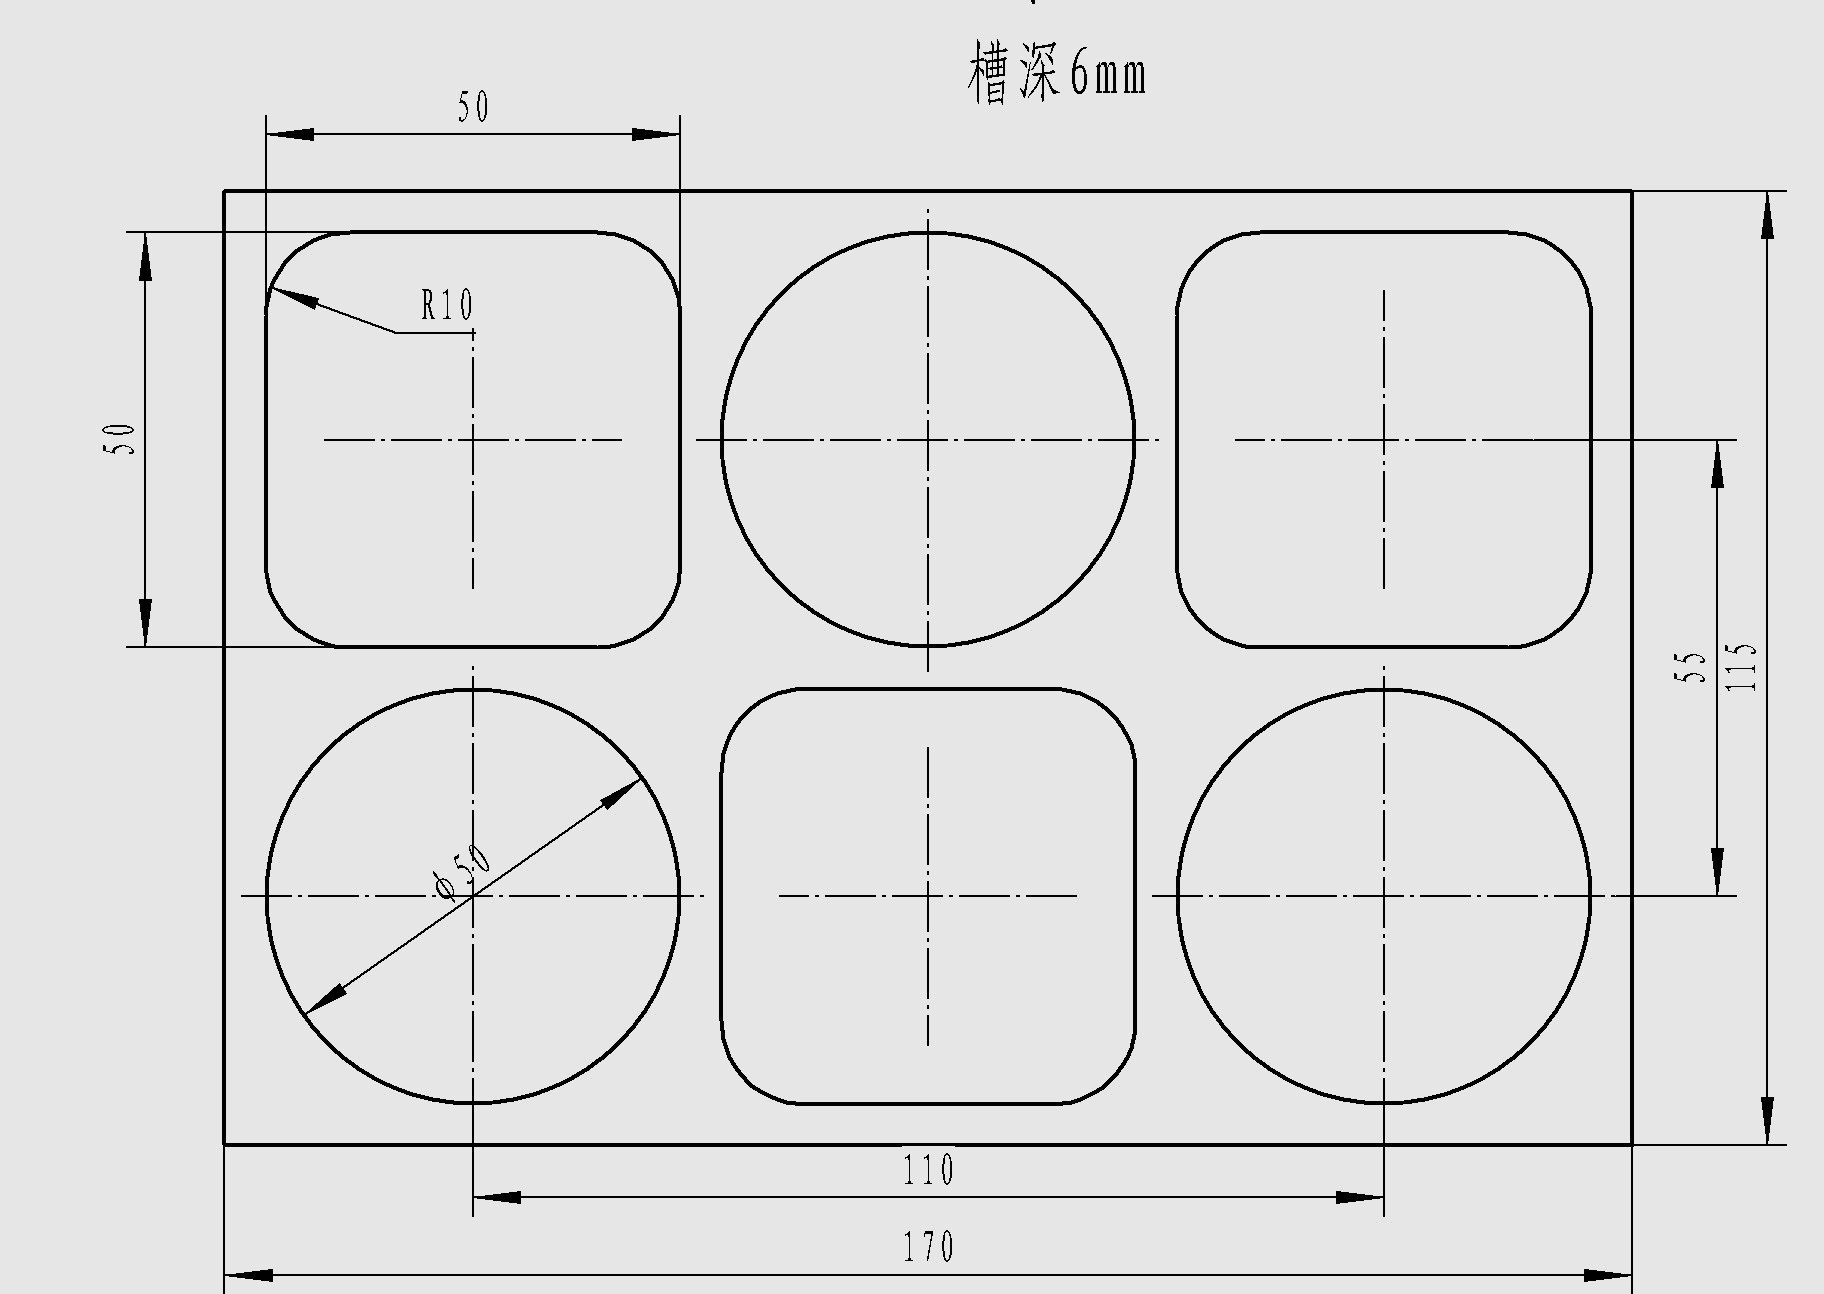
\includegraphics[width=0.8\textwidth]{images/6-1.jpg}
	\caption{局部坐标系} \label{局部坐标系}
\end{figure}

\paragraph{工件坐标系}
\paragraph{装夹}
\paragraph{刀具}
φ12立铣刀

φ8立铣刀
\paragraph{加工顺序}


\subsubsection{应用实例2}
如图\ref{局部坐标系2}所示,加工40*40矩形凸台,高3mm,刀具为Ф14的平底刀。
\begin{figure}[!hbtp]
	\centering	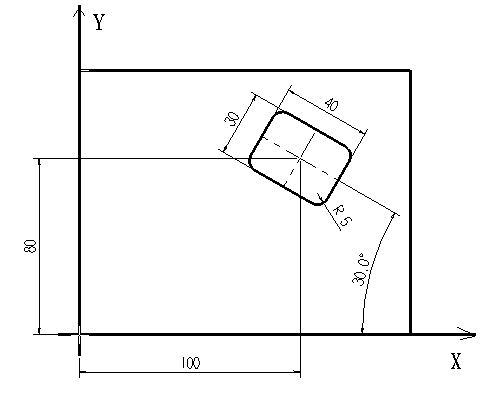
\includegraphics[width=0.8\textwidth]{images/6-2}
	\caption{局部坐标系2} \label{局部坐标系2}
\end{figure}

分析:
\begin{itemize}
\item 凸台为倾斜形式,可以使用旋转指令编程。
\item 凸台四角带圆角,可以使用倒圆角指令编程。
\item 使用局部坐标系,将当前工件坐标系移至凸台的中心处。
\end{itemize}
加工程序如下:
\begin{verbatim}
O1(FANUC)
G54G17G90G40
G01Z100F2000
M03S500
G52X100Y80 当前工件坐标系移至凸台的中心处
G68X0Y0R-30 当前工件坐标系顺时针旋转30度
G00X-35Y0
G01Z-3F1000            
G01G41X-30Y-10D01
G03X-20Y0R10
G01Y15,R5 倒圆角R5
X20,R5
Y-15,R5
X-20,R2
Y0
G03X-30Y10R10
G01G40X-35Y0
G01Z100F2000
G69 取消坐标系旋转
G52X0Y0 取消坐标系平移
M05
M30
\end{verbatim}



\subsection{课堂小结}
\begin{enumerate}[1、]
	\item 几种坐标系;
	\item Fanuc 上的局部坐标系;
	\item Siemens 上的局部坐标系;
	\item 编程实例。
\end{enumerate}

\vfill
\subsection{布置作业}
\begin{enumerate}[1、]
	\item 综合习题一。 
\end{enumerate}
\vfill